%% It is just an empty TeX file.
%% Write your code here.
% !TEX encoding = UTF-8 Unicode
\documentclass[a4paper, 12pt]{article}   	% use "amsart" instead of "article" for AMSLaTeX format
\usepackage[left=20mm, top=15mm, right=10mm, bottom=15mm]{geometry}    

            
\usepackage[parfill]{parskip}    		% Activate to begin paragraphs with an empty line rather than an indent
\usepackage{graphicx}				% Use pdf, png, jpg, or eps§ with pdflatex; use eps in DVI mode
\usepackage[14pt]{extsizes}
\usepackage{setspace,amsmath}
\usepackage{mathtools}
\usepackage{ dsfont }
\usepackage{amsmath,amssymb}
\usepackage[unicode]{hyperref}

\usepackage{xcolor}
\usepackage{color}
\usepackage{minted}
\usepackage{caption}

\usepackage{array}
\newcolumntype{P}[1]{>{\centering\arraybackslash}p{#1}}

\usepackage{cmap} % Улучшенный поиск русских слов в полученном pdf-файле
\usepackage[T2A]{fontenc} % Поддержка русских букв
\usepackage[utf8]{inputenc} % Кодировка utf8
\usepackage[english, russian]{babel} % Языки: русский, английский

								% TeX will automatically convert eps --> pdf in pdflatex		
\usepackage{amssymb}

\begin{document}
\begin{titlepage}

\thispagestyle{empty}

\begin{center}
Федеральное государственное бюджетное образовательное учреждение высшего профессионального образования Московский государственный технический университет имени Н.Э. Баумана
\end{center}


\vfill

\centerline{\large{Лабораторная работа №4. Вариант 1.}}

\centerline{\large{«Методы многомерного поиска.}} 
\centerline{\large{Методы 0-го, 1-го и 2-го порядка»}}

\centerline{\large{по курсу}}
\centerline{\large{«Методы оптимизации»}}


\vfill

Студент группы ИУ9-82 \hfill Белогуров А.А.

Преподаватель \hfill Каганов Ю.T. 
\vfill

\centerline{Москва, 2018}
\clearpage
\end{titlepage}

\newpage
\setcounter{page}{2}

\tableofcontents

\newpage

\section{Цель работы}

\begin{enumerate}
    \item Изучение алгоритмов многомерного поиска.
    \item Разработка программ реализации алгоритмов многомерного поиска 0-го, 1-го  и 2-го порядка.
    \item Вычисление экстремумов функции. 
\end{enumerate}

\newpage

\section{Постановка задачи}
    \textbf {Дано}: 1 Вариант. Функция Розенброка на множестве $R^2$:
    \begin{equation}
        f(x) = \sum^{n-1}_{i=1}{[a(x_i^2 - x_{i+1})^2 + b(x_i - 1)^2] + f_0},
    \end{equation}
    
    где 
    \begin{equation}
        a = 50, \quad b = 2, \quad f_0 = 10, \quad n = 2,
    \end{equation}
    
    тогда функция $f(x)$ будет выглядеть следующим образом:
    \begin{equation}
        f(x) = 50 * (x_0^2 - x_1)^2 + 2 * (x_0 - 1)^2 + 10
    \end{equation}

\subsection{Задача 4.1}
    \begin{enumerate}
        \item Найти экстремум методами:
        \begin{enumerate}
            \item Конфигураций (метод Хука-Дживса).
            \item Нелдера-Мида.
        \end{enumerate}
        \item Найти все стационарные точни и значения функций, соотвестсвующие этим точкам. 
        \item Оценить скорость сходимости указанных алгоритмов.
        \item Реализовать алгоритмы с помощью языка программирования высокого уровня.
    \end{enumerate}
    
    
\subsection{Задача 4.2}
    \begin{enumerate}
        \item Найти экстремум методами:
        \begin{enumerate}
            \item Наискорейшего градиентного спуска.
            \item Флетчера-Ривза.
            \item Девидона-Флетчера-Пауэлла.
            \item Левенберга-Марквардта
        \end{enumerate}
        \item Найти все стационарные точни и значения функций, соотвестсвующие этим точкам. 
        \item Оценить скорость сходимости указанных алгоритмов.
        \item Реализовать алгоритмы с помощью языка программирования высокого уровня.
    \end{enumerate}

\newpage
\section{Исследование}
    Найдем глобальные экстремумы функции 
    \begin{equation}
         f(x) = 50(x_0^2 - x_1)^2 + 2(x_0 - 1)^2 + 10
    \end{equation}
    с помощью сервиса WolframAlpha.com:
    
     \begin{equation}
        min(f(x)) = 10,\quad (x_0, x_1) = (1, 1)
    \end{equation}
    
    \begin{center}
        \begin{minipage}{0.7\linewidth}
            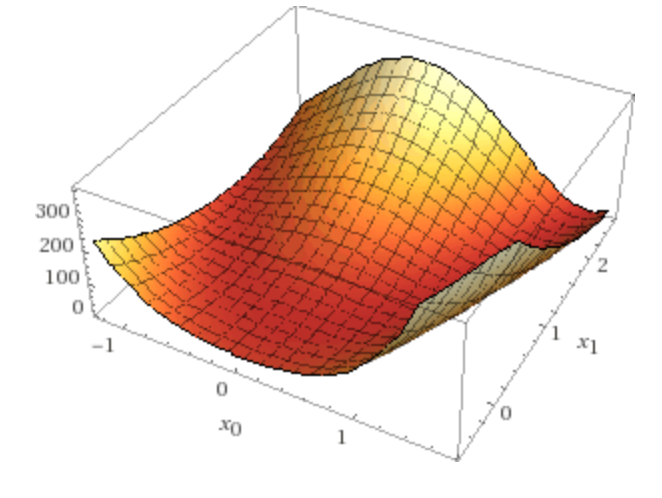
\includegraphics[width=\linewidth]{img/function}
            \captionof{figure}{График функции $f(x)$}
        \end{minipage}
    \end{center}
    
\subsection{Задача 4.1}

\subsubsection{Метод конфигураций (метод Хука-Дживса).}
    Метод конфигураций предназначен для решения задач оптимизации целевой функции многих переменных, при этом целевая функция не обязательно гладкая. Этот метод представляет собой комбинацию исследующего поиска с циклическим изменением переменных и ускоряющего поиска по образцу. Исследующий поиск ориентирован на выявление локального поведения целевой функции и определения направления её убывания вдоль «оврагов». Полученная информация используется при поиске по образцу при движении вдоль «оврагов».
    
\subsubsection{Метод Нелдера-Мида.}
    Метод Нелдера — Мида, также известный как метод деформируемого многогранника и симплекс-метод, — метод безусловной оптимизации функции от нескольких переменных, не использующий производной (точнее — градиентов) функции, а поэтому легко применим к негладким и/или зашумлённым функциям.

    Суть метода заключается в последовательном перемещении и деформировании симплекса вокруг точки экстремума. Метод находит локальный экстремум и может «застрять» в одном из них. Если всё же требуется найти глобальный экстремум, можно пробовать выбирать другой начальный симплекс. Более развитый подход к исключению локальных экстремумов предлагается в алгоритмах, основанных на методе Монте-Карло, а также в эволюционных алгоритмах.
    
\subsection{Задача 4.2}

\subsubsection{Метод наискорейшего градиентного спуска.}
    Стратегия решения задачи состоит в построении последовательности точек $x^k, k=0, 1$ таких, что $f(x^{k+1}0 < f(x^k)$. Точки последовательности ${x^k}$  вычисляются по правилу  $x^{k+1} = x^k - \alpha ^k \bigtriangledown f(x^k)$, где точка $x^0$ задается пользователем; величина шага $\alpha ^k$ определяется для каждого значения  из условия: $\phi (\alpha ^k) = f(x^k - \alpha ^ k \bigtriangledown f(x^k)) \rightarrow \min_{\alpha ^ k}$.

\subsubsection{Метод Флетчера-Ривза.}
    Стратегия метода Флетчера-Ривза состоит в построении последовательности точек ${x^k}$, таких, что $f(x^{k+1}0 < f(x^k)$. Точки последовательности ${x^k}$ вычисляются по правилу:
    \begin{equation}
        x^{k+1} = x^k + \alpha ^k d^l
    \end{equation}
    \begin{equation}
        d ^k = - \bigtriangledown f(x^k) + w ^ {k-1} d ^{k-1}
    \end{equation}
    \begin{equation}
        d^0 = - \bigtriangledown f(x^0)
    \end{equation}
    \begin{equation}
        w^{k-1} = \frac{|| \bigtriangledown f(x^k)||^2}{|| \bigtriangledown f(x^{k-1})||^2}
    \end{equation}
    
    Точка  задается пользователем, величина шага $\alpha ^ k$ определяется для каждого значения k из условия $\alpha ^ k = Arg \min_{\alpha \in R} f(x^k + \alpha ^ k d^ k)$. Решение задачи одномерной минимизации может осуществляться либо из условия $\frac{d \phi (\alpha ^k)}{d \alpha ^k} = 0, \frac{d^ 2 \phi (\alpha ^ k)}{d \alpha ^{k ^ 2}}$ , либо численно, с использованием методов многомерной минимизации, когда решается задача:
	$\phi (\alpha ^ k) \rightarrow \min_{\alpha ^ k \in [a, b]}$.

\subsubsection{Метод Девидона-Флетчера-Пауэлла.}
    Стратегия метода Девидона-Флетчера-Пауэлла состоит в построении последовательности точек ${x^k}$, таких, что $f(x^{k+1}) < f(x^k)$. Точки последовательности ${x^k}$ вычисляются по правилу $x^{k+1} = x^k - \alpha ^k G^{k+1} \bigtriangledown f (x^k)$, где $G^{k+1}$ - матрица размера nxn, являющаяся аппроксимацией обратной матрицы Гессе.

\subsubsection{Метод Левенберга-Марквардта.}
    Стратегия метода Левенберга-Марквардта состоит в построении последовательности точек ${x^k}$, таких, что $f(x^{k+1}) < f(x^k)$. Точки последовательности  ${x^k}$ вычисляются по правилу 
    \begin{equation}
        x^{k+1} = x^k - [H(x) + \mu ^k E]^{-1} \bigtriangledown f(x^k),
    \end{equation}
    где  точка $x^0$ задается пользователем, E - единичная матрица, $\mu ^k$ - последовательность положительных чисел, таких, что матрица  $[H(x) + \mu ^k E]^{-1}$ положительно определена. 

\newpage

\section{Практическая реализация}

    Все методы были реализованы на языке программирования \textbf{Kotlin}. 

\subsection{Задача 4.1}

    \textbf{Листинг 1.} Метод конфигураций.
    \begin{minted}[frame=single, framesep=10pt, fontsize = \footnotesize, linenos=true, breaklines]{kotlin}
fun hookeJeeves(xStart: List<Double>,
                eps: Double,
                function: (xValues: Matrix<Double>) -> Double,
                gradient: (xValues: Matrix<Double>) -> Matrix<Double>) {
    PrintUtils.printInfoStart("Hooke Jeeves")

    var xk = create(xStart.toDoubleArray())
    var k = 0

    while (true) {
        val gradientMat = gradient(xk)

        if (gradientMat.normF() < eps || k >= maxIterations) {
            PrintUtils.printInfoEndFunction(k, 0, xk, function)
            return
        }

        var t = 0.0
        var minValueFun = function(xk - t * gradientMat)

        var i = 0.0
        do {
            i += eps

            val funValue = function(xk - i * gradientMat)
            if (funValue < minValueFun) {
                minValueFun = funValue
                t = i
            }
        } while (i < 2.0)

        val xkNew = xk - t * gradientMat

        if ((xkNew - xk).normF() < eps) {
            PrintUtils.printInfoEndFunction(k, 0, xk, function)
            return
        } else {
            k += 1
            xk = xkNew
        }
    }
}
    \end{minted}

    \textbf{Листинг 2.} Метод Нелдера-Мида.
    \begin{minted}[frame=single, framesep=10pt, fontsize = \footnotesize, linenos=true, breaklines]{kotlin}
fun nelderMead(xStart: List<Double>,
               epsilon: Double,
               stepSize: Double,
               function: (xValues: Matrix<Double>) -> Double) {
    PrintUtils.printInfoStart("Nedler Mead")
    val alpha = 1
    val gamma = 2
    val sigma = -0.5
    val beta = 0.5

    var k = 0

    var v1 = doubleArrayOf(0.0, 0.0)
    var v2 = doubleArrayOf(1.0, 0.0)
    var v3 = doubleArrayOf(0.0, 0.1)

    do {
        k += 1

        var adict = mapOf(
                Pair(v1, function(create(v1))),
                Pair(v2, function(create(v2))),
                Pair(v3, function(create(v3))))

        var points = adict.toList()
                .sortedBy { (_, value) -> value }
                .toMap()

        var b = doubleArrayOf()
        var g = doubleArrayOf()
        var w = doubleArrayOf()
        points.keys.forEachIndexed { index, doubles ->
            when (index) {
                0 -> b = doubles
                1 -> g = doubles
                2 -> w = doubles
            }
        }

        val mid = plusArrays(b, g).map { it -> it / 2 }.toDoubleArray()

        // reflection
        val xr = plusArrays(mid, subArrays(mid, w).map { it -> it * alpha }.toDoubleArray())
        if (function(create(xr)) < function(create(g))) {
            w = xr
        } else {
            if (function(create(xr)) < function(create(w))) {
                w = xr
            }
            val c = plusArrays(w, mid).map { it -> it / 2 }.toDoubleArray()
            if (function(create(c)) < function(create(w))) {
                w = c
            }
        }

        if (function(create(xr)) < function(create(b))) {
            // expansion
            val xe = plusArrays(mid, subArrays(xr, mid).map { it -> it * gamma }.toDoubleArray())
            w = if (function(create(xe)) < function(create(xr))) {
                xe
            } else {
                xr
            }
        }

        if (function(create(xr)) < function(create(g))) {
            // contraction
            val xc = plusArrays(mid, subArrays(w, mid).map { it -> it * beta }.toDoubleArray())

            if (function(create(xc)) < function(create(w))) {
                w = xc
            }
        }

        v1 = w
        v2 = g
        v3 = b
    } while (k < maxIterationsNedlerMead)

    PrintUtils.printInfoEndFunction(k, 0, create(v3), function)
}
    \end{minted}
    
\subsection{Задача 4.2}
    \textbf{Листинг 3.} Метод наискорейшего градиентного спуска.
    \begin{minted}[frame=single, framesep=10pt, fontsize = \footnotesize, linenos=true, breaklines]{kotlin}
fun gradientDescend(xStart: List<Double>,
                    eps: Double,
                    function: (xValues: Matrix<Double>) -> Double,
                    gradient: (xValues: Matrix<Double>) -> Matrix<Double>) {
    PrintUtils.printInfoStart("Gradient Descend")

    var xk = create(xStart.toDoubleArray())
    var k = 0

    while (true) {
        val gradientMat = gradient(xk)

        if (gradientMat.normF() < eps || k >= maxIterations) {
            PrintUtils.printInfoEndFunction(k, 0, xk, function)
            return
        }

        val t = goldenSectionMethod(eps, Interval(0.0, 0.0), xk, gradientMat, function, ::functionHelpValue)

        val xkNew = xk - t * gradientMat

        if ((xkNew - xk).normF() < eps) {
            PrintUtils.printInfoEndFunction(k, 0, xk, function)
            return
        } else {
            k += 1
            xk = xkNew
        }
    }
}
\end{minted}

\textbf{Листинг 4.} Метод Флетчера-Ривза.
    \begin{minted}[frame=single, framesep=10pt, fontsize = \footnotesize, linenos=true, breaklines]{kotlin}
fun flatherRivz(xStart: List<Double>,
                eps: Double,
                function: (xValues: Matrix<Double>) -> Double,
                gradient: (xValues: Matrix<Double>) -> Matrix<Double>,
                isDebug: Boolean) {
    if (isDebug) {
        PrintUtils.printInfoStart("Flatcher-Rivz")
    }

    var xk = create(xStart.toDoubleArray())
    var xkOld = create(xStart.toDoubleArray())
    var xkNew = create(xStart.toDoubleArray())

    var k = 0
    var d = create(doubleArrayOf())

    while (true) {
        val gradientMat = gradient(xk)

        if (gradientMat.normF() < eps || k >= maxIterations) {
            PrintUtils.printInfoEndFunction(k, 0, xk, function)
            return
        }

        if (k == 0) {
            d = -gradientMat
        }

        val betta = gradient(xkNew).normF() / gradient(xkOld).normF()
        val dNew = - gradient(xkNew) + betta * d

        val t = goldenSectionMethod(eps, Interval(0.0, 0.0), xk, gradientMat, function, ::functionHelpValue)

        xkNew = xk + t * dNew

        if ((xkNew - xk).normF() < eps) {
            PrintUtils.printInfoEndFunction(k, 0, xk, function)
            return
        } else {
            k += 1
            xkOld = xk
            xk = xkNew
            d = dNew
        }
    }
}
\end{minted}

\textbf{Листинг 5.} Метод Девидона-Флетчера-Пауэлла.
    \begin{minted}[frame=single, framesep=10pt, fontsize = \footnotesize, linenos=true, breaklines]{kotlin}
fun davidonFlatcherPowell(xStart: List<Double>,
                          eps: Double,
                          function: (xValues: Matrix<Double>) -> Double,
                          gradient: (xValues: Matrix<Double>) -> Matrix<Double>) {
    PrintUtils.printInfoStart("Davidon-Flatcher-Powell")

    var xk = create(xStart.toDoubleArray())
    var xkOld = create(xStart.toDoubleArray())
    var xkNew = create(xStart.toDoubleArray())

    var k = 0
    var A = eye(2)

    while (true) {
        val gradientMat = gradient(xk)

        if (gradientMat.normF() < eps || k >= maxIterations) {
            PrintUtils.printInfoEndFunction(k, 0, xk, function)
            return
        }

        if (k != 0) {
            val deltaG = gradient(xk) - gradient(xkOld)
            val deltaX = xk - xkOld

            var A_C = (deltaX * deltaX.T).elementSum() / (deltaX.T * deltaG).elementSum()
            A_C -= (multiplyMatrices(A, deltaG) * multiplyMatrices(A.T, deltaG.T)).elementSum() / (multiplyMatrices(deltaG.T, A) * deltaG).elementSum()

            A += A_C
        }

        val t = goldenSectionMethod(eps, Interval(0.0, 0.0), xk, gradientMat, function, ::functionHelpValue)

        xkNew = xk - t * multiplyMatrices(A, gradientMat)
        if ((xkNew - xk).normF() < eps && (function(xkNew) - function(xk)).absoluteValue < eps) {
            PrintUtils.printInfoEndFunction(k, 0, xk, function)
        } else {
            k += 1
            xkOld = xk
            xk = xkNew
        }
    }

}
\end{minted}

\textbf{Листинг 6.} Метод Левенберга-Марквардта.
    \begin{minted}[frame=single, framesep=10pt, fontsize = \footnotesize, linenos=true, breaklines]{kotlin}
fun levenbergMarkvardt(xStart: List<Double>,
                        eps: Double,
                        function: (xValues: Matrix<Double>) -> Double,
                        gradient: (xValues: Matrix<Double>) -> Matrix<Double>,
                        hessian: (xValues: Matrix<Double>) -> Matrix<Double>) {
    PrintUtils.printInfoStart("Levenberg-Markvardt")
    
    var xk = create(xStart.toDoubleArray())
    
    var k = 0
    var nu = 10.pow(4)
    
    while (true) {
        val gradientMat = gradient(xk)
    
        if (gradientMat.normF() < eps || k >= maxIterations) {
            PrintUtils.printInfoEndFunction(k, 0, xk, function)
            return
        }
    
        while (true) {
            val hessianMat = hessian(xk)
    
            val temp = hessianMat + nu * eye(2)
            val tempInv = temp.inv()
    
            val dK = - multiplyMatrices(tempInv, gradientMat)
    
            val xkNew = xk + dK
    
            if (function(xkNew) < function(xk)) {
                k += 1
                nu /= 2
                xk = xkNew
                break
            } else {
                nu *= 2
            }
        }
    }
}
\end{minted}

    
\newpage

\section{Результаты.}
    При последовательном запуске всех алгоритмов со следующими параметрами -
    \begin{equation}
        epsilon = 10^{-4}
    \end{equation}
    были получены следующие результаты:
    
    \textbf{Листинг 7.} Результаты выполнения программ.
    \begin{minted}[frame=single, framesep=10pt, fontsize = \footnotesize, linenos=true, breaklines]{text}
Start Hooke Jeeves:
	 Iteration(s): 104
	 f(mat[ 1.0096764585235,  1.01948882952882 ]) = 10.000187357073251

Start Nedler Mead:
	 Iteration(s): 23
	 f(mat[ 0.99162736535072,  0.98263914436102 ]) = 10.000163710379134

Start Gradient Descend:
	 Iteration(s): 691
	 f(mat[ 0.98948881136718,  0.97880461881578 ]) = 10.000224988473748

Start Flatcher-Rivz:
	 Iteration(s): 18
	 f(mat[ 0.99994078064943,  0.99990294247419 ]) = 10.000000029864099

Start Davidon-Flatcher-Powell:
	 Iteration(s): 380
	 f(mat[ 0.99999952984738,  0.99999881907983 ]) = 10.000000000003336


Start Levenberg-Markvardt:
	 Iteration(s): 3014
	 f(mat[ 0.99999409370002,  0.99998767059015 ]) = 10.000000000083125
	 \end{minted}
 
Все результаты с небольшой погрешностью совпадают с результатами полученными с помощью сервиса WolframAlpha.com в пункте 3. 

\end{document} 